\documentclass{scrreprt}

\usepackage[english,ngerman]{babel} 
\usepackage[utf8]{inputenc} 
\usepackage{graphicx}
\usepackage{dsfont}
\usepackage{amsmath}

\title{TH1 - Aufgabenblatt 2}
\author{Andreas Krohn, Erik Andresen, Benjamin Vetter, Andreas Basener}

\begin{document}

\maketitle

\begin{enumerate}

\item Welche Eigenschaften sollte Eure Gleisanlage haben? (informelle Beschreibung)

\begin{itemize}
  \item Deadlock-Freiheit
  \item Starvation-Frei
  \item Beschränkt bzgl. der maximalen Anzahl an fahrenden Zügen pro Gleisabschnitt
  \item Kollisionsfrei
  \item Alpenpanorama
\end{itemize}

\item Modellierung:

(a) Modelliert die einzelnen o.g. Gleise, Weichen und die Schranke jeweils mit
    einem eigenen S/T-Netz. Wie werden die Züge darin modelliert?

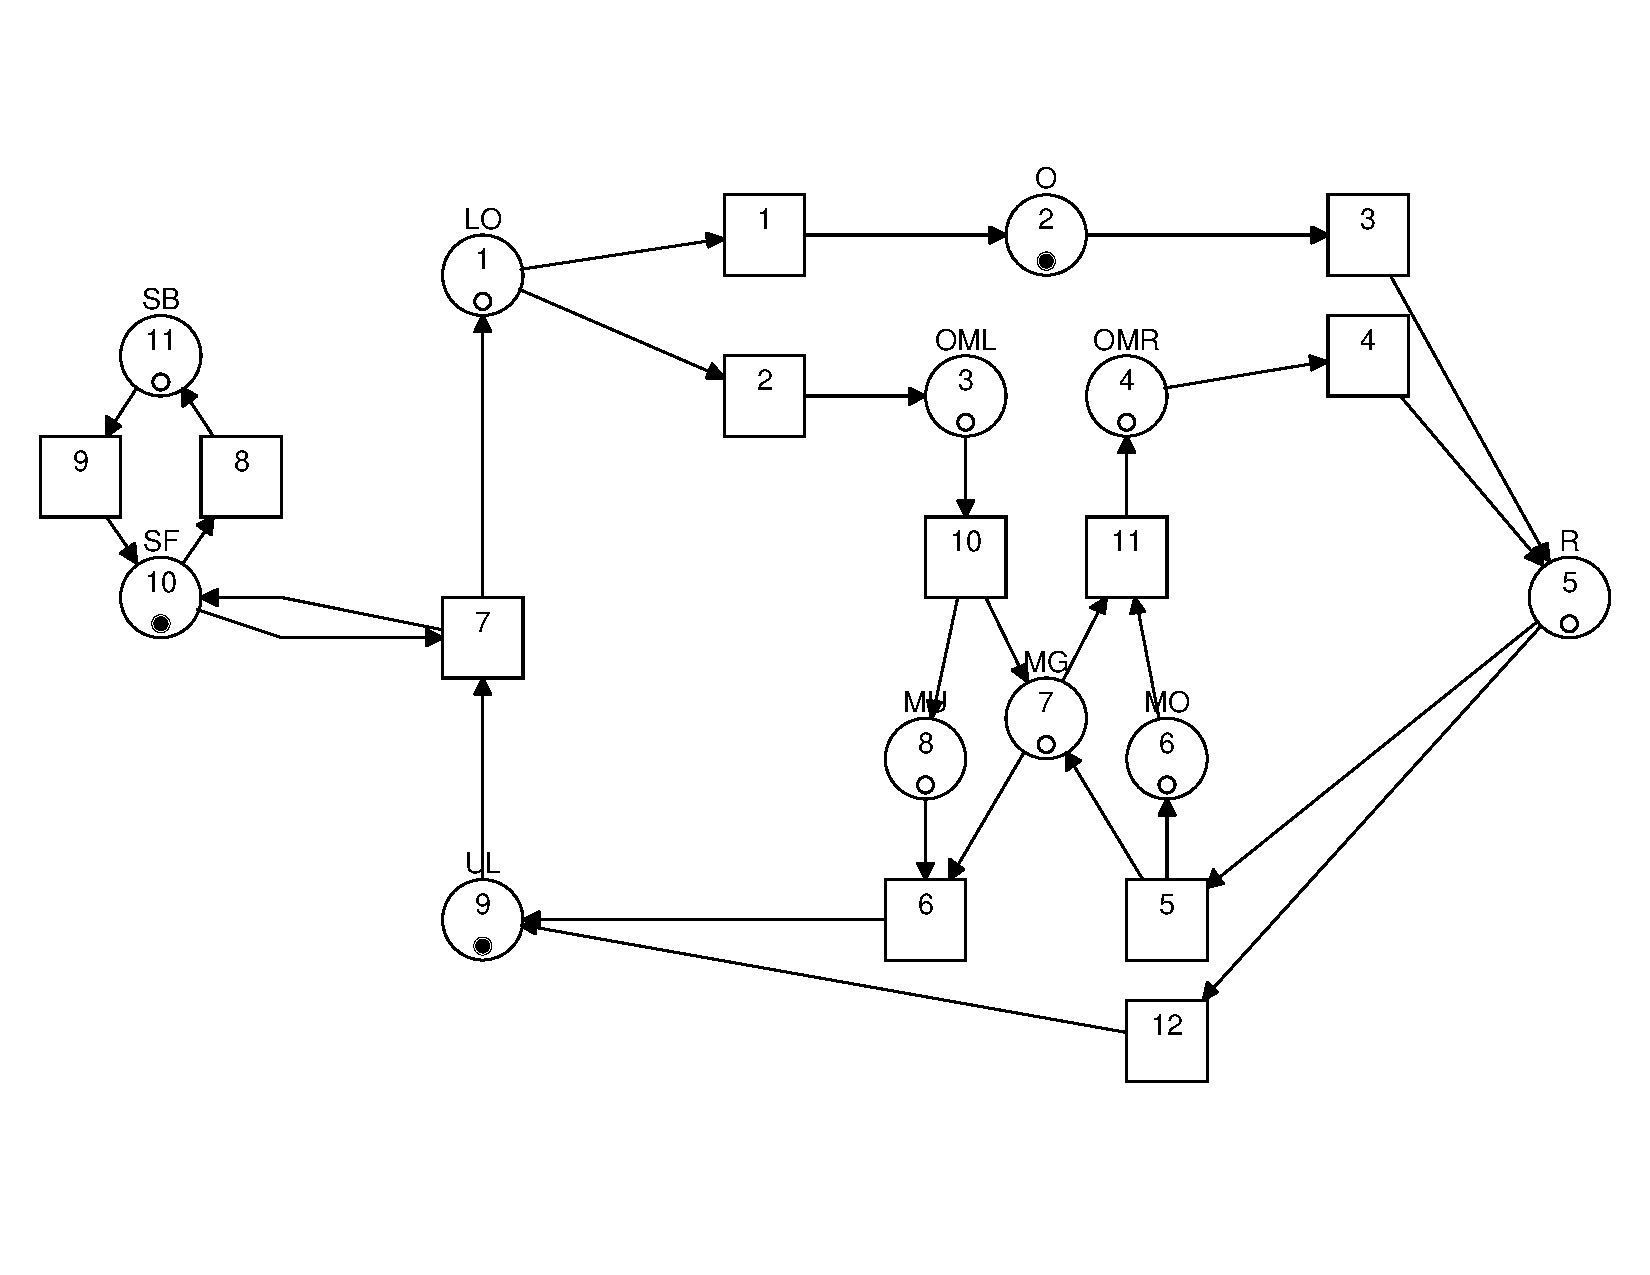
\includegraphics[width=1\textwidth]{prak2_aufg2.pdf}
\end{enumerate}

\end{document}

